\section{Specifica dei casi d'uso}
In questa sezione si analizzeranno le classi e come sono relazionate tra loro, daremo un'occhiata ai sequence diagram (in particolare quelli riguardanti due funzionalità dell'applicazione) e agli statechart relativi all'interfaccia grafica. Per fare ciò utilizzeremo:
\begin{enumerate}
  \item Class diagram.
  \item Sequence diagram.
  \item State chart
\end{enumerate}
\subsection{Classi, oggetti e relazioni di analisi}
In questa sezione utilizzeremo i \textit{class diagram} per farci un idea della relazione tra le classi, prima di tutto diamo uno sguardo alla struttura generale che abbiamo creato in fase di analisi:
\begin{figure}[H]
  \centering
  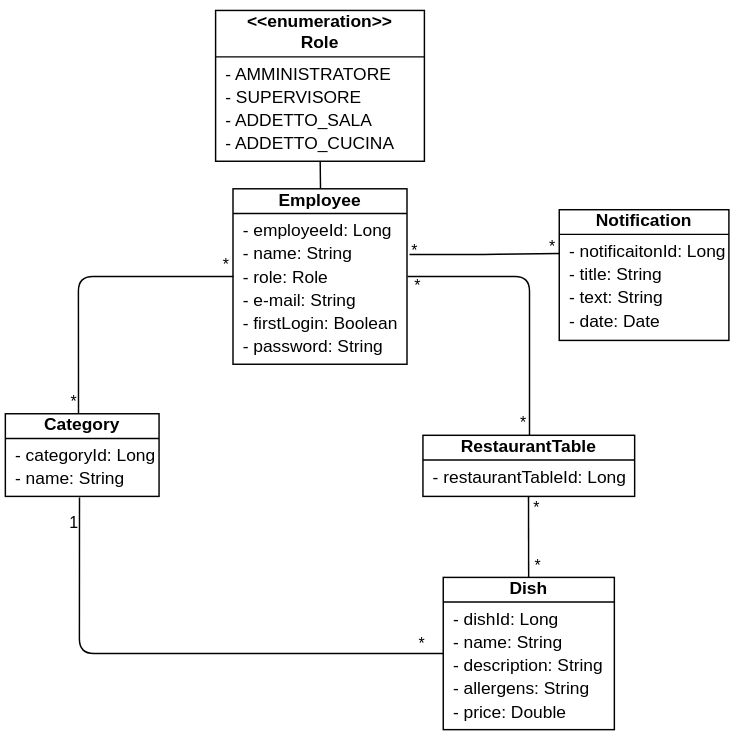
\includegraphics[scale=0.6]{img/class_diagrams/generalClassDiagram.png}
  \caption{Class diagram delle entità}
\end{figure}
D'ora in poi invece, i \textit{class diagram} mostrati, saranno quelli delle funzionalità che sono state assegnate al team di sviluppo.
\newpage
\subsection{Class diagram di analisi - Gestione menù}
In questo class diagram viene analizzato il punto 3 della traccia ovvero la gestione del menù.
\begin{figure}[H]
  \centering
  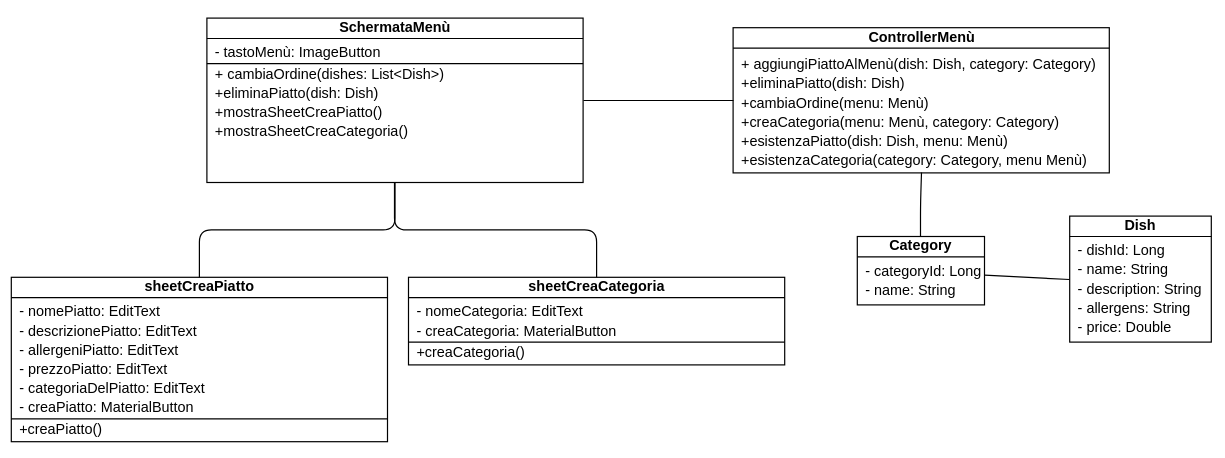
\includegraphics[scale=0.55]{img/class_diagrams/gestioneMenu_class_diagram.png}
  \caption{Class diagram della gestione del menù}
\end{figure}
\newpage
\subsection{Class diagram - Creazione utenza}
Nel seguente class diagram verrà analizzato il punto 1, quello nel quale si richiede la creazione di un utente e l'eventuale cambio password nel caso in cui si tratti del primo login, il cambio password verrà però affrontato in un \textit{class diagram} successivo, in modo da poter comprendere anche l'accesso alla piattaforma.

\begin{figure}[H]
  \centering
  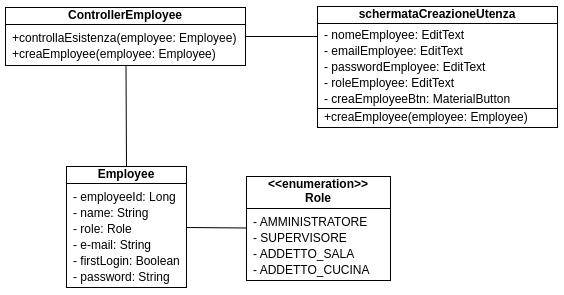
\includegraphics[scale=0.75]{img/class_diagrams/creazioneUtenza_class_diagram.png}
  \caption{Class diagram per la creazione utenze}
\end{figure}
\subsubsection{Class diagram - Accesso alla piattaforma}
Adesso, come detto in precedenza, analizzeremo l'accesso (con conseguente cambio password) alla piattaforma.
\begin{figure}[H]
  \centering
  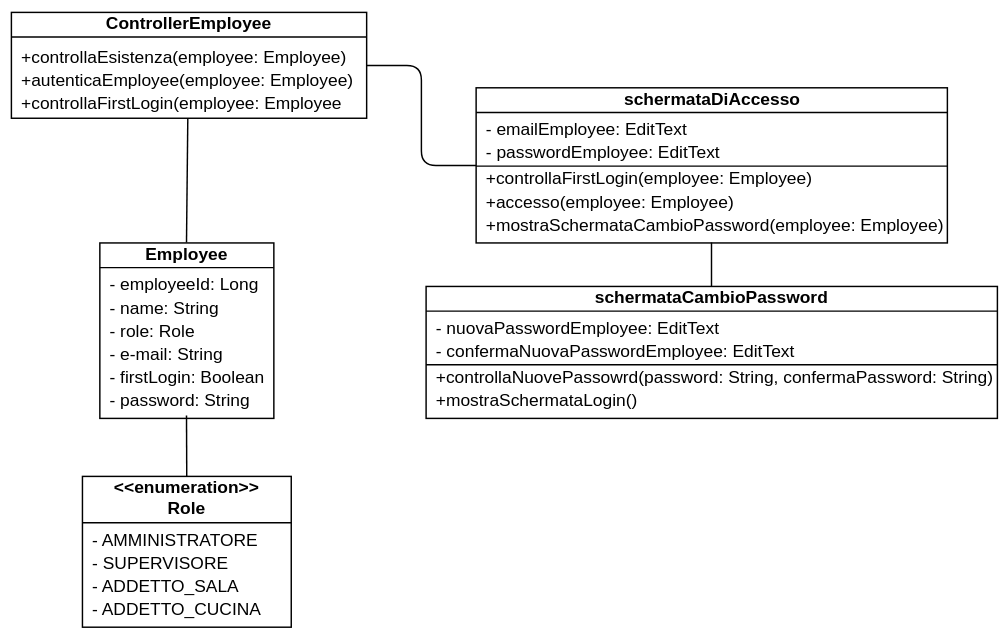
\includegraphics[scale=0.5]{img/class_diagrams/accessoCambioPassword_class_diagram.png}
  \caption{Class diagram dell'accesso alla piattaforma}
\end{figure}
\subsection{Class diagram - Gestione tavoli}
Il seguente \textit{class diagram} analizza il punto 6, quindi creazione ordinazioni indicando l'identificativo del tavolo e gli elementi del menù da aggiungere al tavolo.
\begin{figure}[H]
  \centering
  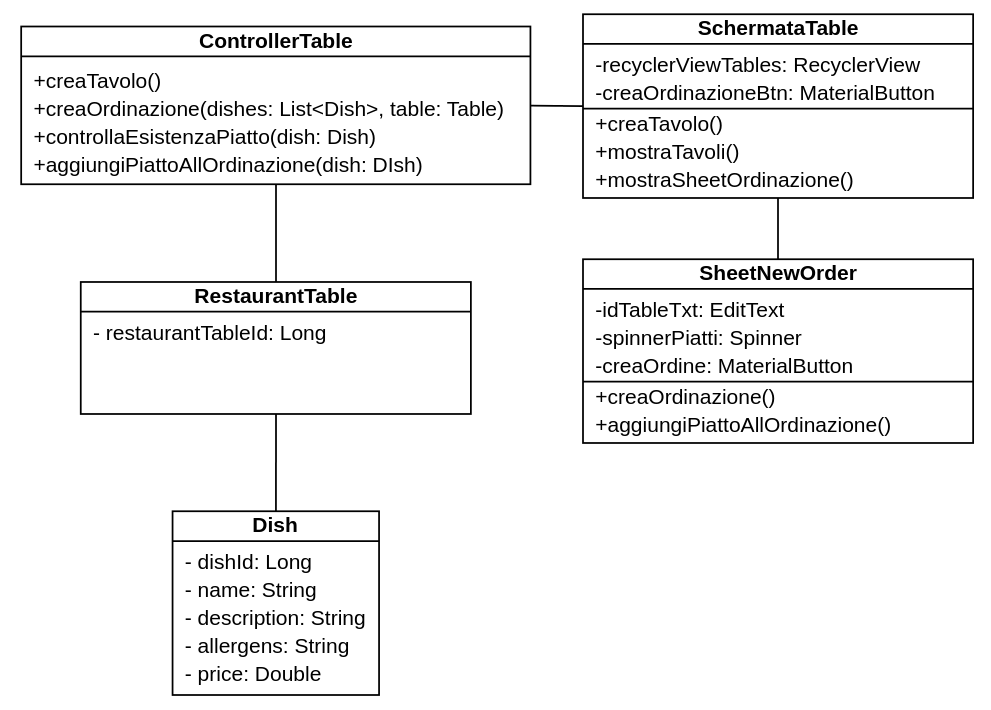
\includegraphics[scale=0.5]{img/class_diagrams/gestioneTavoli_class_diagram.png}
  \caption{Class diagram della gestione dei tavoli}
\end{figure}
\newpage
\subsection{Class diagram - Gestione notifiche}
Il seguente \textit{class diagram} analizza il punto 13, quindi creazione di avvisi (notifiche), al quale verrà aggiunta la visualizzazione delle notifiche.
\begin{figure}[H]
  \centering
  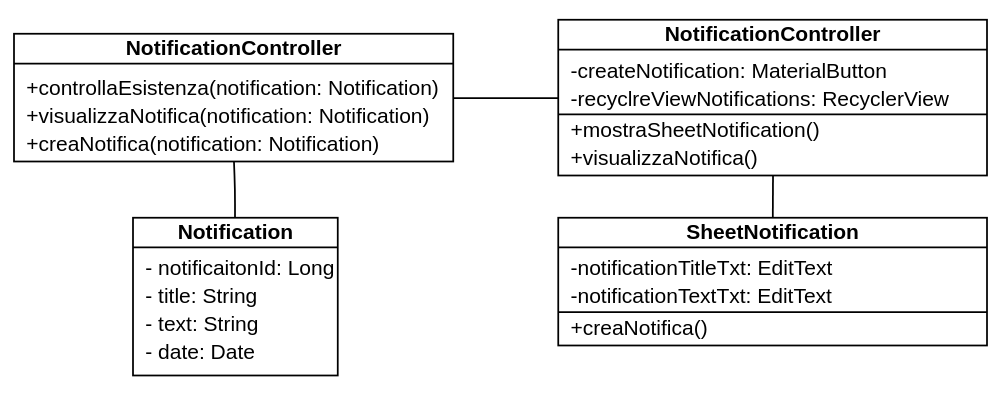
\includegraphics[scale=0.5]{img/class_diagrams/gestioneNotifiche_class_diagram.png}
  \caption{Class diagram della gestione delle notifiche}
\end{figure}
